\chapter{\luDecompTitle}
\label{LUdecomp}

Certain matrices are easier to work with than others.  In this section, we will see how to write any square\footnote{The case where $M$ is not square is dealt with at the end of the lecture.} matrix $M$ as the product of two simpler matrices.  We will write \[M=LU\, ,\] where:
\begin{itemize}
\item $L$ is \emph{lower triangular}\index{Lower triangular matrix}.  This means that all entries above the main diagonal are zero.  In notation,
$L=(l^i_j)$ with $l^i_j=0$ for all $j>i$.
\[L=\begin{pmatrix}
l^1_1 & 0 & 0 & \cdots \\
l^2_1 & l^2_2 & 0 & \cdots \\
l^3_1 & l^3_2 & l^3_3 & \cdots \\
\vdots & \vdots & \vdots & \ddots \\
\end{pmatrix}
\]

\item $U$ is \emph{upper triangular}\index{Upper triangular matrix}.  This means that all entries below the main diagonal are zero.  In notation,
$U=(u^i_j)$ with $u^i_j=0$ for all $j<i$.
\[U=\begin{pmatrix}
u^1_1 & u^1_2 & u^1_3 & \cdots \\
0 & u^2_2 & u^2_3 & \cdots \\
0 & 0 & u^3_3 & \cdots \\
\vdots & \vdots & \vdots & \ddots \\
\end{pmatrix}
\]
\end{itemize}
$M=LU$ is called an \emph{$LU$ decomposition}\index{LU@$LU$ decomposition} of $M$.

This is a useful trick for  computational reasons; it is much easier to compute the inverse of an upper or lower triangular matrix than general matrices.  Since inverses are useful for solving linear systems, this makes solving any linear system associated to the matrix much faster as well.  The determinant---a very important quantity associated with any square matrix---is very easy to compute for triangular matrices.

\begin{example}
Linear systems associated to upper triangular matrices are very easy to solve by back substitution.
\[
\begin{amatrix}{2}
a & b & 1 \\
0 & c & e \\
\end{amatrix} \ \Rightarrow \ y=\frac{e}{c}\, , \quad x=\frac{1}{a}\left(1-\frac{be}{c}\right)
\]

\[
\begin{amatrix}{3}
1 & 0 & 0 & d \\
a & 1 & 0 & e \\
b & c & 1 & f \\
\end{amatrix} \Rightarrow x=d\, , \qquad y=e-ad\, , \qquad z=f-bd-c(e-ad)
\]
For lower triangular matrices, \emph{back} substitution\index{Back substitution} gives a quick solution; for upper triangular matrices, \emph{forward} substitution\index{Forward substitution} gives the solution.
\end{example}





\section{Using $LU$ Decomposition to Solve Linear Systems}

Suppose we have $M=LU$ and want to solve the system
\[
MX=LUX=V.
\]

\begin{itemize}
\item{Step 1:} Set $W=\colvec{u\\v\\w}=UX$.  

\item{Step 2:} Solve the system $LW=V$.  This should be simple by forward substitution since $L$ is lower triangular.  Suppose the solution to $LW=V$ is $W_0$.  

\item{Step 3:} Now solve the system $UX=W_0$.  This should be easy by backward substitution, since $U$ is upper triangular.  The solution to this system is the solution to the original system.
\end{itemize}
We can think of this as using the matrix $L$ to perform row operations on the matrix $U$ in order to solve the system; this idea also appears in the  study of determinants.

%\href{\webworkurl ReadingHomework11/1/}{Reading homework: problem 11.1}
\reading{11}{1}

\begin{example}
Consider the linear system:
\[
      \begin{linsys}{4}
            6x & +&18y & +&3z         &=& 3  \\[1mm]
            2x & +&12y & +&z	    &=& 19 \\[1mm]
            4x & +&15y & +&3z         &=& 0  
      \end{linsys}
\]

An $LU$ decomposition for the associated matrix $M$ is:
\[
\begin{pmatrix}
6 & 18 & 3 \\
2 & 12 & 1 \\
4 & 15 & 3 
\end{pmatrix} =
\begin{pmatrix}
3 & 0 & 0 \\
1 & 6 & 0 \\
2 & 3 & 1 
\end{pmatrix}
\begin{pmatrix}
2 & 6 & 1 \\
0 & 1 & 0 \\
0 & 0 & 1 
\end{pmatrix}.
\]

\begin{itemize}
\item{Step 1:} \hypertarget{LUproc}{Set} $W=\colvec{u\\v\\w}=UX$.  

\item{Step 2:} Solve the system $LW=V$:

\[
\begin{pmatrix}
3 & 0 & 0 \\
1 & 6 & 0 \\
2 & 3 & 1 
\end{pmatrix}
\colvec{u\\v\\w} =
\colvec{3\\19\\0}
\]

By substitution, we get $u=1$, $v=3$, and $w=-11$.  Then 
\[W_0=\colvec{1\\3\\-11}\]

\item{Step 3:} Solve the system $UX=W_0$.  
\[
\begin{pmatrix}
2 & 6 & 1 \\
0 & 1 & 0 \\
0 & 0 & 1 
\end{pmatrix}
\colvec{x\\y\\z} =
\colvec{1\\3\\-11}
\]
Back substitution gives $z=-11, y=3$, and $x=-3$.  

Then $X=\colvec{-3\\3\\-11}$, and we're done.
\end{itemize}
\end{example}

\videoscriptlink{lu_decomposition_using_lu_decomp.mp4}{Using a $LU$ decomposition}{scripts_lu_decomposition_using_lu_example}

%\begin{figure}
\begin{center}
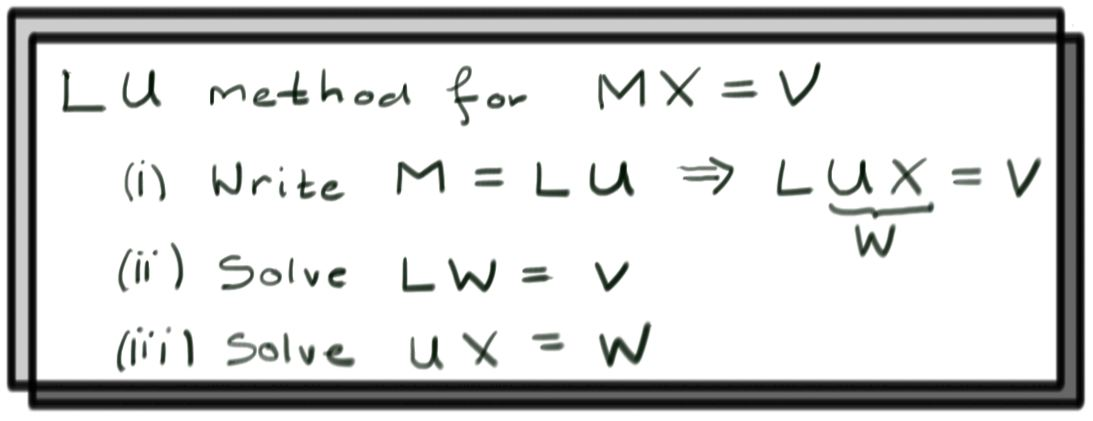
\includegraphics[scale=.3]{\luDecompPath/LU_solution.jpg}
\end{center}
%\end{figure}

\section{Finding an $LU$ Decomposition.}
\label{finding_LU_decomp}
 
For any given matrix, there are actually many different $LU$ decompositions.  However, there is a unique $LU$ decomposition in which the $L$ matrix has ones on the diagonal. In that case $L$ is called a \emph{lower unit triangular matrix}\index{Lower unit triangular matrix}.

To find the $LU$ decomposition, we'll create two sequences of matrices $L_0, L_1, \ldots$ and $U_0, U_1, \ldots$ such that at each step, $L_iU_i=M$.  Each of the $L_i$ will be lower triangular, but only the last $U_i$ will be upper triangular.

Start by setting $L_0=I$ and $U_0=M$, because $L_0U_0=M$. A main concept of this calculation is captured by the following example:

\begin{example}
Consider \[E=\begin{pmatrix}1&0\\\lambda&1\end{pmatrix}\, ,\qquad M=\begin{pmatrix}a&b&c&\cdots\\d&e&f&\cdots\end{pmatrix}\, .\]
Lets compute $EM$
\[
EM=\begin{pmatrix}a&b&c&\cdots\\d+\lambda a&e+\lambda b&f+\lambda c&\cdots\end{pmatrix}\, ,.
\]
Something neat happened here: multiplying $M$ by $E$ performed the row operation $R_2\to R_2+\lambda R-1$ on $M$.
Another interesting fact:
\[
E^{-1}:=\begin{pmatrix}1&0\\-\lambda&1\end{pmatrix}
\] 
obeys (check this yourself...)
\[
E^{-1} E = 1\, .
\]
Hence $M=E^{-1} E M$ or, writing this out
\[
\begin{pmatrix}a&b&c&\cdots\\d&e&f&\cdots\end{pmatrix}=\begin{pmatrix}1&0\\-\lambda&1\end{pmatrix} \begin{pmatrix}a&b&c&\cdots\\d+\lambda a&e+\lambda b&f+\lambda c&\cdots\end{pmatrix}\, .
\]
Here the matrix on the left is lower triangular, while the matrix on the right has had a row operation performed on it.
\end{example}




\vspace{2mm}
We would like to  use the first row of $U_0$ to zero out the first entry of every row below it.  For our running example, \[U_0=M=\begin{pmatrix}
6 & 18 & 3 \\
2 & 12 & 1 \\
4 & 15 & 3 
\end{pmatrix}\, ,\] so we would like to perform the row operations $R_2\to R_2 -\frac 13 R_1$ and $R_3\to R_3-\frac 23R_1$.
%so the second row minus $\frac{1}{3}$ of the first row will zero out the first entry in the second row.  Likewise, the third row minus $\frac{2}{3}$ of the first row will zero out the first entry in the third row.
If we perform these row operations on $U_0$ to produce 
\[U_1=\begin{pmatrix}
6 & 18 & 3 \\
0 & 6 & 0 \\
0 & 3 & 1 
\end{pmatrix}\, ,\]
we need to multiply this on the left by a lower triangular matrix $L_1$ so that the product $L_1U_1=M$ still.
The above example shows how to do this:
Set $L_1$ to be the lower triangular matrix whose first column is filled with the minus constants used to zero out the first column of $M$.  Then \[L_1 = \begin{pmatrix}
1 & 0 & 0 \\[1mm]
\frac{1}{3} & 1 & 0 \\[1mm]
\frac{2}{3} & 0 & 1 
\end{pmatrix}\, .\]  
%Set $U_1$ to be the matrix obtained by zeroing out the first column of $M$.  Then $U_1=\begin{pmatrix}
%6 & 18 & 3 \\
%0 & 6 & 0 \\
%0 & 3 & 1 
%\end{pmatrix}$.
By construction $L_1 U_1=M$, but you should compute this yourself as a double check.

Now repeat the process by zeroing the second column of $U_1$ below the diagonal using the second row of $U_1$ using the row operation
$R_3\to R_3-\frac 12 R_2$ to produce
\[U_2=\begin{pmatrix}6&18&3\\0&6&0\\0&0&1\end{pmatrix}\, .\]
The matrix that undoes this row operation is obtained in the same way we found $L_1$ above and is:
\[
\begin{pmatrix}
1&0&0\\
0&1&0\\
0&\frac 12& 0
\end{pmatrix}\, .
\]
Thus our answer for $L_2$ is the product of this matrix with $L_1$, namely
\[
L_2=
\begin{pmatrix}
1 & 0 & 0 \\[1mm]
\frac{1}{3} & 1 & 0 \\[1mm]
\frac{2}{3} & 0 & 1 
\end{pmatrix}\begin{pmatrix}
1&0&0\\
0&1&0\\
0&\frac 12& 0
\end{pmatrix}
=\begin{pmatrix}
1 & 0 & 0 \\[1mm]
\frac{1}{3} & 1 & 0 \\[1mm]
\frac{2}{3} & \frac{1}{2} & 1 
\end{pmatrix}\, .
\]
Notice that it is lower triangular because 

\begin{center}
\textcolor{brown}{THE PRODUCT OF LOWER TRIANGULAR MATRICES IS ALWAYS LOWER TRIANGULAR!}
\end{center}

\noindent
Moreover it is obtained by recording minus the constants used for all our row operations in the appropriate columns (this always works this way).
Moreover, $U_2$ is upper triangular and $M=L_2U_2$, we are done!
Putting this all together we have
\[M=\begin{pmatrix}
6 & 18 & 3 \\
2 & 12 & 1 \\
4 & 15 & 3 
\end{pmatrix}= \begin{pmatrix}
1 & 0 & 0 \\[1mm]
\frac{1}{3} & 1 & 0 \\[1mm]
\frac{2}{3} & \frac{1}{2} & 1 
\end{pmatrix}\begin{pmatrix}
6 & 18 & 3 \\
0 & 6 & 0 \\
0 & 0 & 1 
\end{pmatrix}\, .\]  
%Since $U_2$ is upper-triangular, we're done.  Inserting the new number into $L_1$ to get $L_2$ really is safe: the numbers in the first column don't affect the second column of $U_1$, since the first column of $U_1$ is already zeroed out.

If the matrix you're working with has more than three rows, just continue this process by zeroing out the next column below the diagonal, and repeat until there's nothing left to do.

\videoscriptlink{lu_decomposition_example.mp4}{Another $LU$ decomposition example}{scripts_lu_decomposition_example}

The fractions in the $L$ matrix are admittedly ugly.  For two matrices $LU$, we can multiply one entire column of $L$ by a constant $\lambda$ and divide the corresponding row of $U$ by the same constant without changing the product of the two matrices.  Then:

\begin{eqnarray*}
LU &=& \begin{pmatrix}
1 & 0 & 0 \\[1mm]
\frac{1}{3} & 1 & 0 \\[1mm]
\frac{2}{3} & \frac{1}{2} & 1 
\end{pmatrix}
I
\begin{pmatrix}
6 & 18 & 3 \\
0 & 6 & 0 \\
0 & 0 & 1 
\end{pmatrix} \\
&=&
\begin{pmatrix}
1 & 0 & 0 \\[1mm]
\frac{1}{3} & 1 & 0 \\[1mm]
\frac{2}{3} & \frac{1}{2} & 1 
\end{pmatrix}
\begin{pmatrix}
3 & 0 & 0 \\
0 & 6 & 0 \\
0 & 0 & 1 
\end{pmatrix}
\begin{pmatrix}
\frac{1}{3} & 0 & 0 \\[1mm]
0 & \frac{1}{6} & 0 \\[1mm]
0 & 0 & 1 
\end{pmatrix}
\begin{pmatrix}
6 & 18 & 3 \\
0 & 6 & 0 \\
0 & 0 & 1 
\end{pmatrix} \\
&=&
\begin{pmatrix}
3 & 0 & 0 \\
1 & 6 & 0 \\
2 & 3 & 1 
\end{pmatrix}\begin{pmatrix}
2 & 6 & 1 \\
0 & 1 & 0 \\
0 & 0 & 1 
\end{pmatrix}.
\end{eqnarray*}
The resulting matrix looks nicer, but isn't in standard (lower unit triangular matrix) form.

\reading{11}{2}
%\href{\webworkurl ReadingHomework11/2/}{Reading homework: problem 11.2}

For matrices that are not square, $LU$ decomposition still makes sense.  Given an $m\times n$ matrix $M$, for example we could write $M=LU$ with $L$ a square lower unit triangular matrix, and $U$ a rectangular matrix.  Then $L$ will be an $m\times m$ matrix, and $U$ will be an $m\times n$ matrix (of the same shape as $M$).  From here, the process is exactly the same as for a square matrix.  We create a sequence of matrices $L_i$ and $U_i$ that is eventually the $LU$ decomposition.  Again, we start with $L_0=I$ and $U_0=M$.

\begin{example}
Let's find the $LU$ decomposition of $M=U_0=\begin{pmatrix}
-2 & 1 & 3 \\
-4 & 4 & 1 
\end{pmatrix}$.  Since $M$ is a $2\times 3$ matrix, our decomposition will consist of a $2\times 2$ matrix and a $2\times 3$ matrix.  Then we start with $L_0=I_2=\begin{pmatrix}
1 & 0 \\
0 & 1
\end{pmatrix}$.

The next step is to zero-out the first column of $M$ below the diagonal.  There is only one row to cancel, then, and it can be removed by subtracting $2$ times the first row of $M$ to the second row of $M$.  Then:

\[
L_1=\begin{pmatrix}
1 & 0 \\
2 & 1
\end{pmatrix}, \qquad 
U_1 = \begin{pmatrix}
-2 & 1 & 3 \\
0 & 2 & -5 
\end{pmatrix}
\]
Since $U_1$ is upper triangular, we're done.  With a larger matrix, we would just continue the process.
\end{example}





\section{Block $LDU$ Decomposition}

Let $M$ be a square block matrix with square blocks $X,Y,Z,W$ such that $X^{-1}$ exists.  Then $M$ can be decomposed as a block $LDU$ decomposition, where $D$ is block diagonal, as follows:
\[
M=\begin{pmatrix}
X & Y \\
Z & W
\end{pmatrix}
\]

Then: \[M=\begin{pmatrix}
I &  0 \\
ZX^{-1} & I
\end{pmatrix}\begin{pmatrix}
X & 0 \\
0 & W-ZX^{-1}Y
\end{pmatrix}\begin{pmatrix}
I & X^{-1}Y \\
0 & I
\end{pmatrix}.\]
This can be checked explicitly simply by block-multiplying these three matrices.

\videoscriptlink{lu_decomposition_blocks.mp4}{Block $LDU$ Explanation}{scripts_lu_decomposition_blocks}

\begin{example}
For a $2\times 2$ matrix, we can regard each entry as a block.
\[
\begin{pmatrix}
1 & 2 \\
3 & 4
\end{pmatrix}=
\begin{pmatrix}
1 & 0 \\
3 & 1
\end{pmatrix}
\begin{pmatrix}
1 & 0 \\
0 & -2
\end{pmatrix}
\begin{pmatrix}
1 & 2 \\
0 & 1
\end{pmatrix}
\]
By multiplying the diagonal matrix by the upper triangular matrix, we get the standard $LU$ decomposition of the matrix.
\end{example}


%\section*{References}
%Wikipedia:
%\begin{itemize}
%\item \href{http://en.wikipedia.org/wiki/LU_decomposition}{$LU$ Decomposition}
%\item \href{http://en.wikipedia.org/wiki/Block_LU_decomposition}{Block $LU$ Decomposition}
%\end{itemize}

\section{Review Problems}




\begin{enumerate}
\item \label{det33} Let $M=\begin{pmatrix}
m^1_1 & m^1_2 & m^1_3\\
m^2_1 & m^2_2 & m^2_3\\
m^3_1 & m^3_2 & m^3_3\\
\end{pmatrix}$.  Use row operations to put $M$ into \emph{row echelon form}.  For simplicity, assume that $m_1^1\neq 0 \neq m^1_1m^2_2-m^2_1m^1_2$.

Prove that $M$ is non-singular if and only if:
\[
m^1_1m^2_2m^3_3 
- m^1_1m^2_3m^3_2 
+ m^1_2m^2_3m^3_1 
- m^1_2m^2_1m^3_3 
+ m^1_3m^2_1m^3_2
- m^1_3m^2_2m^3_1
\neq 0
\]

\phantomnewpage

\item 
\begin{enumerate}
\item What does the matrix $E^1_2=\begin{pmatrix}
0 & 1 \\
1 & 0
\end{pmatrix}$ do to $M=\begin{pmatrix}
a & b \\
d & c
\end{pmatrix}$ under left multiplication?  What about right multiplication?
\item Find elementary matrices $R^1(\lambda)$ and $R^2(\lambda)$ that respectively multiply rows $1$ and $2$ of $M$ by $\lambda$ but otherwise leave $M$ the same under left multiplication.
\item Find a matrix $S^1_2(\lambda)$ that adds a multiple $\lambda$ of row $2$ to row $1$ under left multiplication.
\end{enumerate}

\phantomnewpage

\item Let $M$ be a matrix and $S^i_jM$ the same matrix with rows \(i\) and \(j\) switched.  Explain every line of the 
\hyperlink{rowswap}{series of equations} proving that $\det M = -\det (S^i_jM)$.

\phantomnewpage

%\item \label{prob_inversion_number} This problem is a ``hands-on'' look at why \hyperlink{permutation_parity}{the property} describing the parity of permutations is true.
%
%\hypertarget{inversion_number}{The \emph{inversion number}}\index{Permutation!Inversion number} of a permutation $\sigma$ is the number of pairs $i<j$ such that $\sigma(i)>\sigma(j)$; it's the number of ``numbers that appear left of smaller numbers'' in the permutation.  For example, for the permutation $\rho = [4,2,3,1]$, the inversion number is $5$. The number $4$ comes before $2,3,$ and $1$, and $2$ and $3$ both come before $1$.
%
%Given a permutation $\sigma$, we can make a new permutation $\tau_{i,j} \sigma$ by exchanging the $i$th and $j$th entries of $\sigma$.
%
%\begin{enumerate}
%\item What is the inversion number of the permutation \(\mu=[1,2,4,3]\) that exchanges 4 and 3 and leaves everything else alone? Is it an even or an odd permutation?
%
%\item What is the inversion number of the permutation \(\rho=[4,2,3,1]\) that exchanges 1 and 4 and leaves everything else alone? Is it an even or an odd permutation?
%
%\item What is the inversion number of the permutation \(\tau_{1,3} \mu\)? Compare the parity\footnote{The \emph{parity} of an integer refers to whether the integer is even or odd. Here the parity of a permutation $\mu$ refers to the parity of its inversion number.} of \(\mu\) to the parity of \(\tau_{1,3} \mu.\)
%
%\item What is the inversion number of the permutation \(\tau_{2,4} \rho\)? Compare the parity of \(\rho\) to the parity of \(\tau_{2,4} \rho.\)
%
%\item What is the inversion number of the permutation \(\tau_{3,4} \rho\)? Compare the parity of \(\rho\) to the parity of \(\tau_{3,4} \rho.\)
%\end{enumerate}
%
%\videoscriptlink{elementary_matrices_determinant_hint.mp4}{Problem~\ref{prob_inversion_number} hints}{scripts_elementary_matrices_determinants_hint}

\phantomnewpage

%\item \label{problem_permutation} (Extra credit) Here we will examine a (very) small set of the general properties about permutations and their applications. In particular, we will show that one way to compute the sign of a permutation is by finding the \hyperlink{inversion_number}{inversion number} $N$ of $\sigma$ and we have
%\[
%\sgn(\sigma) = (-1)^N.
%\]
%
%For this problem, let $\mu = [1,2,4,3]$.
%
%\begin{enumerate}
%\item Show that every permutation $\sigma$ can be sorted by only taking simple (adjacent) transpositions\index{Permutation!Simple transposition} $s_i$ where $s_i$ interchanges the numbers in position $i$ and $i+1$ of a permutation $\sigma$ (in our other notation $s_i = \tau_{i,i+1}$). For example $s_2 \mu = [1, 4, 2, 3]$, and to sort $\mu$ we have $s_3 \mu = [1, 2, 3, 4]$.
%
%\item \label{prob_part_relations} We can compose simple transpositions together to represent a permutation (note that the sequence of compositions is not unique), and these are associative, we have an identity (the trivial permutation where the list is in order or we do nothing on our list), and we have an inverse since it is clear that $s_i s_i \sigma = \sigma$. Thus permutations of $[n]$ under composition are an example of a \hyperref[groups]{group}. However note that not all simple transpositions commute with each other since
%\begin{align*}
%s_1 s_2 [1, 2, 3] & = s_1 [1, 3, 2] = [3, 1, 2]
%\\ s_2 s_1 [1, 2, 3] & = s_2 [2, 1, 3] = [2, 3, 1]
%\end{align*}
%(you will prove here when simple transpositions commute). When we consider our initial permutation to be the trivial permutation $e = [1, 2, \dotsc, n]$, we do not write it; for example $s_i \equiv s_i e$ and $\mu = s_3 \equiv s_3 e$. This is analogous to not writing 1 when multiplying. Show that $s_i s_i = e$ (in shorthand $s_i^2 = e$), $s_{i+1} s_i s_{i+1} = s_i s_{i+1} s_i$ for all $i$, and $s_i$ and $s_j$ commute for all $|i - j| \geq 2$.
%
%\item Show that every way of expressing $\sigma$ can be obtained from using the relations proved in part~\ref{prob_part_relations}. In other words, show that for any expression $w$ of simple transpositions representing the trivial permutation $e$, using the proved relations.
%
%\emph{Hint: Use induction on $n$. For the induction step, follow the path of the $(n+1)$-th strand by looking at $s_n s_{n-1} \cdots s_k s_{k\pm1} \cdots s_n$ and argue why you can write this as a subexpression for any expression of $e$. Consider using diagrams of these paths to help.}
%
%\item The simple transpositions \hyperlink{action}{acts on} an $n$-dimensional vector space $V$ by $s_i v = E^i_{i+1} v$ (where $E^i_j$ is \hyperlink{elem_matrix_row_swap}{an elementary matrix}) for all vectors $v \in V$. Therefore we can just represent a permutation $\sigma$ as the matrix $M_{\sigma}$\footnote{Often people will just use $\sigma$ for the matrix when the context is clear.}, and we have $\det(M_{s_i}) = \det(E^i_{i+1}) = -1$. Thus prove that $\det(M_{\sigma}) = (-1)^N$ where $N$ is a number of simple transpositions needed to represent $\sigma$ as a permutation. You can assume that $M_{s_i s_j} = M_{s_i} M_{s_j}$ (it is not hard to prove) and that $\det(A B) = \det(A) \det(B)$ \hyperref[detmultiplicative]{from Chapter~\ref*{elementarydeterminantsII}}.
%
%\emph{Hint: You to make sure $\det(M_{\sigma})$ is well-defined since there are infinite ways to represent $\sigma$ as simple transpositions.}
%
%\item Show that $s_{i+1} s_i s_{i+1} = \tau_{i, i+2}$, and so give one way of writing $\tau_{i, j}$ in terms of simple transpositions? Is $\tau_{i,j}$ an even or an odd permutation? What is $\det(M_{\tau_{i,j}})$? What is the inversion number of $\tau_{i,j}$?
%
%\item The minimal number of simple transpositions needed to express $\sigma$ is called the \emph{length}\index{Permutation!Length} of $\sigma$; for example the length of $\mu$ is 1 since $\mu = s_3$. Show that the length of $\sigma$ is equal to the inversion number of $\sigma$.
%
%\emph{Hint: Find an procedure which gives you a new permutation $\sigma^{\prime}$ where $\sigma = s_i \sigma^{\prime}$ for some $i$ and the inversion number for $\sigma^{\prime}$ is 1 less than the inversion number for $\sigma$.}
%
%\item Show that $(-1)^N = \sgn(\sigma) = \det(M_{\sigma})$, where $\sigma$ is a permutation with $N$ inversions. Note that this immediately implies that $\sgn(\sigma \rho) = \sgn(\sigma) \sgn(\rho)$ for any permutations $\sigma$ and $\rho$.
%\end{enumerate}

\item Let $M'$ be the matrix obtained from $M$ by swapping two columns $i$ and $j$. Show that $\det M'=-\det M $.

\item The scalar triple product of three vectors $u,v,w$ from $\Re^3$ is $u\cdot(v\times w)$. Show that this product is the same as the determinant of the matrix whose columns are $u,v,w$ (in that order). What happens to the scalar triple product when the factors are permuted? 

\item Show that if $M$ is a $3\times 3$ matrix whose third row is a sum of multiples of the other rows ($R_3=aR_2+bR_1$) then $\det M=0$. Show that the same is true if one of the columns is a sum of multiples of the others. 

\end{enumerate}

\phantomnewpage

\newpage
